
\documentclass[10pt]{article}

\usepackage{graphicx}
\usepackage{amsmath,amsfonts,amssymb}

\usepackage{hyperref}  % for urls and hyperlinks


\setlength{\textwidth}{6.2in}
\setlength{\oddsidemargin}{0.3in}
\setlength{\evensidemargin}{0in}
\setlength{\textheight}{8.9in}
\setlength{\voffset}{-1in}
\setlength{\headsep}{26pt}
\setlength{\parindent}{0pt}
\setlength{\parskip}{5pt}



% a few handy macros

\newcommand\matlab{{\sc matlab}}
\newcommand{\goto}{\rightarrow}
\newcommand{\bigo}{{\mathcal O}}
\newcommand{\half}{\frac{1}{2}}
%\newcommand\implies{\quad\Longrightarrow\quad}
\newcommand\reals{{{\rm l} \kern -.15em {\rm R} }}
\newcommand\complex{{\raisebox{.043ex}{\rule{0.07em}{1.56ex}} \hskip -.35em {\rm C}}}


% macros for matrices/vectors:

% matrix environment for vectors or matrices where elements are centered
\newenvironment{mat}{\left[\begin{array}{ccccccccccccccc}}{\end{array}\right]}
\newcommand\bcm{\begin{mat}}
\newcommand\ecm{\end{mat}}

% matrix environment for vectors or matrices where elements are right justifvied
\newenvironment{rmat}{\left[\begin{array}{rrrrrrrrrrrrr}}{\end{array}\right]}
\newcommand\brm{\begin{rmat}}
\newcommand\erm{\end{rmat}}

% for left brace and a set of choices
\newenvironment{choices}{\left\{ \begin{array}{ll}}{\end{array}\right.}
\newcommand\when{&\text{if~}}
\newcommand\otherwise{&\text{otherwise}}
% sample usage:
%  \delta_{ij} = \begin{choices} 1 \when i=j, \\ 0 \otherwise \end{choices}


% for labeling and referencing equations:
\newcommand{\eql}{\begin{equation}\label}
\newcommand{\eqn}[1]{(\ref{#1})}
% can then do
%  \eql{eqnlabel}
%  ...
%  \end{equation}
% and refer to it as equation \eqn{eqnlabel}.  


% some useful macros for finite difference methods:
\newcommand\unp{U^{n+1}}
\newcommand\unm{U^{n-1}}

% for chemical reactions:
\newcommand{\react}[1]{\stackrel{K_{#1}}{\rightarrow}}
\newcommand{\reactb}[2]{\stackrel{K_{#1}}{~\stackrel{\rightleftharpoons}
   {\scriptstyle K_{#2}}}~}

% Parts:

% set enumerate to give parts a, b, c, ...  rather than numbers 1, 2, 3...
\renewcommand{\theenumi}{\alph{enumi}}
\renewcommand{\labelenumi}{(\theenumi)}

% set second level enumerate to give parts i, ii, iii, iv, etc.
\renewcommand{\theenumii}{\roman{enumii}}
\renewcommand{\labelenumii}{(\theenumii)}




\begin{document}

% header:
\hfill \vbox{
\hbox{AMath 584 / Math 584}
\hbox{Homework \#3}
\hbox{Due 11:00pm PDT}
\hbox{Tuesday, November 8, 2016}
}


\vskip 0.5cm

{\bf Name:}   Your Name Here

{\bf Netid:}  Your NetID Here

\vskip 0.5cm

%--------------------------------------------------------------------------
\vskip 1cm
\hrule
{\bf Problem 1.}
Let
\[
A = \bcm 0&3\\ 2&0\\ 0&4\ecm.
\]

Do this problem ``by hand'', and write out the matrices that you get at
each stage. 

\begin{enumerate}
\item Use the classical Gram-Schmidt algorithm to determine a reduced QR
factorization of $A = \hat Q \hat R$.

\item From this determine the full $QR$ factorization with $Q$ a unitary
$3\times 3$ matrix.

\item Determine a full QR factorization using the Householder
triangularization algorithm.  In particular:
\begin{itemize}
\item Determine the Householder reflector $F_1 = Q_1$ 
that reduces $A$ to the form
\[
Q_1A = \bcm X&X\\ 0&X\\ 0&X \ecm
\] 
where  the $X$'s show elements that are possibly nonzero.  

\item Determine the $2\times 2$ Householder reflector $F_2$ so that
the $3\times 3$ matrix
\[
Q_2 = \bcm 1&0^T\\ 0&F_2 \ecm  \qquad \text{(where $0 \in \reals^2$)}
\]
reduces $Q_1A$ to the desired upper triangular form $Q_2Q_1A = R \in
\reals^{3\times 2}$. 

\item  Determine $Q$ so that $A=QR$ from $Q_1$ and $Q_2$.
\end{itemize} 
This is following the notation used in lecture on Friday October 21.

{\bf Note:} Recall that the choice of $v$ in (10.5) in the book is for
numerical stability and mathematically the first term could be given a plus
or minus sign and the algorithm would work.  In the case when
$x_1=0$, define sign(0) $=1$.

\end{enumerate} 

Comment on whether these two approaches gave the same matrices $Q$ and $R$
and if not what the difference is.


% uncomment the next two lines if you want to insert solution...
%\vskip 1cm
%{\bf Solution:}

% insert your solution here!


%--------------------------------------------------------------------------
\newpage
\vskip 1cm
\hrule
{\bf Problem 2.}
\begin{enumerate} 
\item
Using the results of Problem 1(a) above, determine the (left) pseudoinverse
$A^+$ for the matrix from Problem 1.
\item 
Compute $A^+b$  and $A^+c$ for the two vectors
\[
b = \bcm 3\\2\\4\ecm, \qquad c = \bcm -16\\0\\12 \ecm.
\]
Explain why $A^+c$ gives the zero vector.
\end{enumerate}


% uncomment the next two lines if you want to insert solution...
%\vskip 1cm
%{\bf Solution:}

% insert your solution here!


%--------------------------------------------------------------------------
\vskip 1cm
\hrule
{\bf Problem 3.}
Let $q\in\complex^m$ have $\|q\|_2=1$.  Then $P = qq^*$ is a projection
matrix.
\begin{enumerate} 
\item The matrix $P$ has a singular value decomposition with $U =
[q|Q_\perp]$ for some appropriate matrix $Q_\perp$.
What are the singular values of $P$?

\item Find an SVD of the projection matrix $I-P = I-qq^*$. 
In particular, what are the singluar values?
{\bf Hint:} Write $I=UU^*$ where $U$ is as above and use the SVD of $qq^*$.

\item Find an SVD of the reflector $I-2P$. What are the singular values?
%%% Removed --> Think about the geometric interpretation of these values.

{\bf Modified:}{\em Recall that the singular values should be non-negative.}

\item {\bf Added:}
{\em Suppose you write a
general vector $x$ as a linear combination of the columns of $U$, i.e., as 
$x = c_1u_1 + c_2u_2 + \cdots + c_mu_m$ where $c_j = u_j^*x$.  
In terms of a similar representation using the columns of $U$ as a basis, 
what are the vectors $Px,~ (I-P)x$, and $(I-2P)x$.  Think about the geometric
meaning of these.}

\end{enumerate} 


% uncomment the next two lines if you want to insert solution...
%\vskip 1cm
%{\bf Solution:}

% insert your solution here!


%--------------------------------------------------------------------------
\vskip 1cm
\hrule
{\bf Problem 4.}
Consider the polynomial of Exercise 13.3 in the book, for which
\begin{verbatim}
c = [-512, 2304, -4608, 5376, -4032, 2016, -672, 144, -18, 1]
\end{verbatim} 

\begin{enumerate}
\item Write a function in Matlab or Python {\tt psum(x,c)} that evaluates a
polynomial defined by coefficients {\tt c}  by the natural summation
algorithm, e.g. in pseudo-code:
\begin{verbatim}
    psum = c[0]
    for j = 1 to n-1
        psum = psum + c[j]*t**j
\end{verbatim}
for a polynomial of degree $n-1$.
Test your function to make sure it works on some simple examples.

\item

Put in a print statement to print out the partial sum {\tt psum} each
time through the loop.  Now test it on the polynomial $p(x)$ from Exer. 13.3
at $x = 2.1$.  How large is the error in the computed value?
Comment on how this relates to the size of the partial sums.
{\bf Hint:} The true value is easy to compute from the fact that $p(x) =
(x-2)^9$.

\item Do the same thing using Horner's method to evaluate the polynomial.
Use the Python function given in the
notebook {\tt notebooks/LeastSquares2.ipynb} or write a Matlab version.

\item Plot the polynomial near $x=2$ by evaluating at the points {\tt
linspace(1.95, 2.05, 101)} using both evaluation methods and plot these
curves together. (You will want to take out the print statements for this.)  

Also plot the polynomial when it is evaluated using the
expression $(x-2)^9$.  This should be the most accurate and give a smooth
curve that approximates the true polynomial.
\end{enumerate} 

% uncomment the next two lines if you want to insert solution...
%\vskip 1cm
%{\bf Solution:}

% insert your solution here!

%--------------------------------------------------------------------------
\vskip 1cm
\hrule
{\bf Problem 5.}
Exercise 14.1 in the book.  Briefly explain your answers.

For (d), look up 
\href{https://en.wikipedia.org/wiki/Stirling%27s_approximation}{Stirling's
approximation} for the factorial.

% uncomment the next two lines if you want to insert solution...
%\vskip 1cm
%{\bf Solution:}

% insert your solution here!

\vskip 1cm
\hrule
{\bf Problem 6.}

The file {\tt homeworks/hw3/co2.txt} in the class repository
contains a set of data that you will need for this assignment.  

This file contains 90 lines of comments
followed by 636 lines of data.  The third column is time (in years) and the
fourth column is CO$_2$ concentration in the atmosphere (in parts per
million) as measured at Mauna Loa.  These give a set of $(t_i,~y_i)$ values
that we will apply least squares to.
See \url{http://www.esrl.noaa.gov/gmd/ccgg/trends/mlo.html}
for more information on this data.  
(Note that the file you are using is from 2011, not the most recent version.)

Plotting this data should give:

\centerline{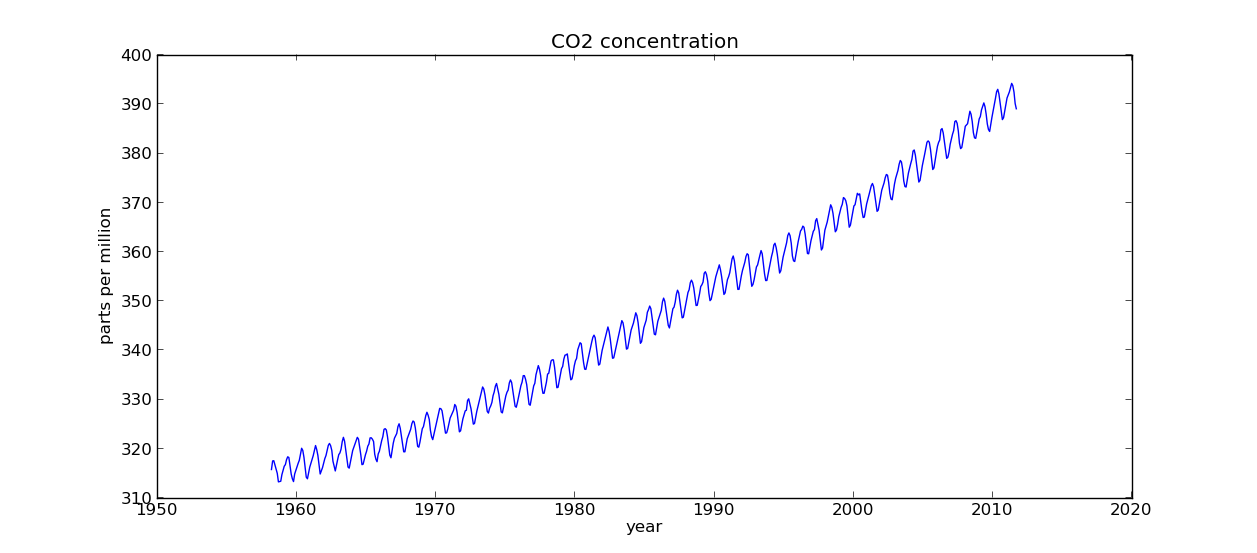
\includegraphics[width=5.5in]{co2figure.png}}

\vskip 5pt
To produce such a plot (and to do the rest of this assignment) you will have
to read the data into Matlab or Python and first pre-process it by stripping
out any $(t,y)$ values for which $y = -99.99$ (indicating that data was not
available at this time).

The codes at the end of the assignment 
show how to do this, and print out the figure as
a {\tt png} file that can be incorporated in your latex as illustrated in
this file.


There is a clear oscillation in this data with a period of one
year, due to seasonal variations.  There is also an upward trend that might
be fit with a linear function as the first attempt.  This suggests we
perform a
least squares fit with the basis functions
\[
\phi_0(t) = \cos(2\pi t), \quad
\phi_1(t) = \sin(2\pi t), \quad
\phi_2(t) = 1, \quad
\phi_3(t) = t-1985. \quad
\]
The shift by 1985 in the last basis function keeps the values in the matrix
smaller, and becomes particularly important when we add higher powers.

{\bf (a)~} 
Use Matlab or Python to compute the least squares fit. 

{\bf Added to assignment:}
{\em 
Do this by computing the QR factorization (using the built-in {\tt qr}
function) and then solving $Rc = Q^Ty$.  In Matlab you can solve this
nonsingular linear system using the backslash operator, 
{\tt c = R\textbackslash Q'*y}.

(Note that in Matlab you can also solve a least square problem directly with
the backslash operator,\\
{\tt c = A\textbackslash b}, 
and in Python the function {\tt numpy.linalg.lstsq(A,b)} can be used.  }

Plot the fit as a red curve on the same plot. 

To see the trend without the oscillation, take the coefficients
$c\in\reals^4$ just found and plot the function
\[
p(t) = c_2\phi_2(t) + c_3\phi_3(t) 
\]
on the same plot, as a green curve.  

Also plot the residual as a function of time on a separate plot.

You should get something like these:

\centerline{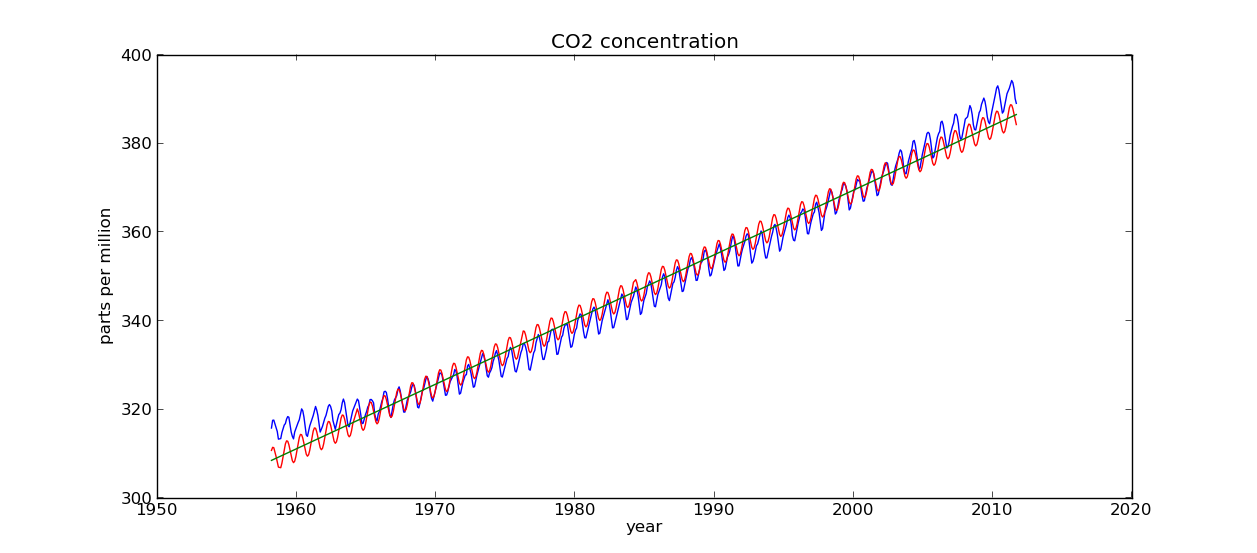
\includegraphics[width=5.5in]{co2figure1.png}}

\centerline{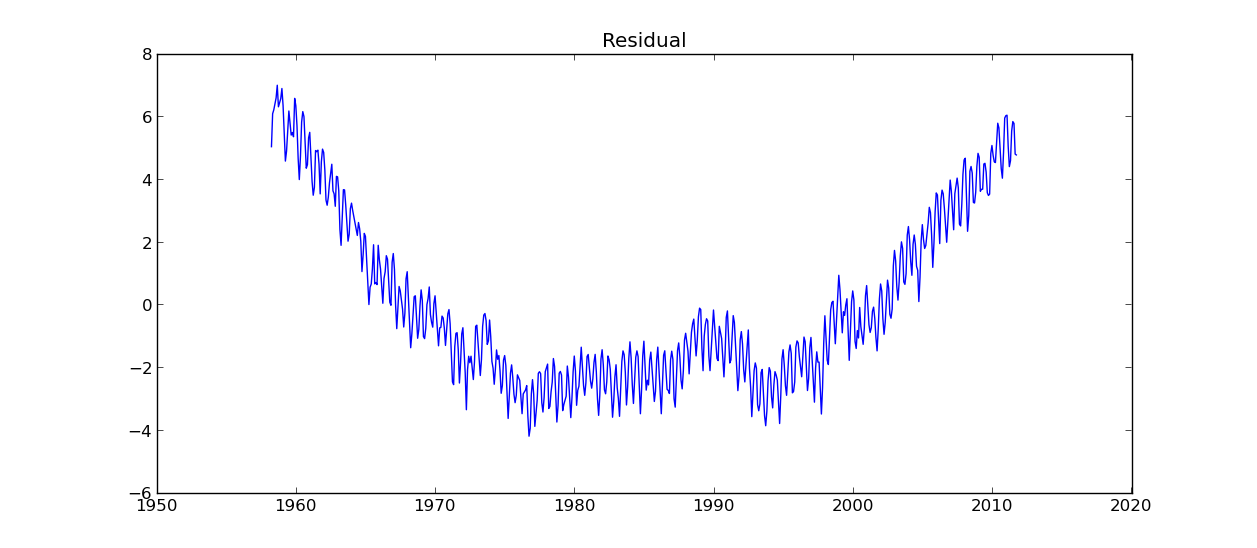
\includegraphics[width=5.5in]{co2resid1.png}}



{\bf (b)~} This fit doesn't match the trend very well, so we might try
improving it by using a quadratic function instead of linear for the
``secular terms'', especially
since the residual looks something like a parabola.  This can be
done by adding another basis function $\phi_4(t) = (t-1985)^2$.  Repeat part
(a) using this.  Plot the fit, the quadratic trend, and the residual.

{\bf (c)~} 
This fit looks good enough that we might be tempted to use it to predict the
future.  Evaluate the function $f(t)$ over the interval $1960 \leq t \leq
2050$ with enough points to show how it behaves and plot this.

As a sanity check we might also try extrapolating backwards in time.  Plot
the same function $f(t)$ over the interval $1800 \leq t \leq 2010$ and
comment on what you see.  

\newpage
{\large\bf Matlab:}

\begin{verbatim}

% Read column data with whitespace delimiter, skipping 90 rows:
d = importdata('co2.txt',' ',90)
data = d.data;
t = data(:,3);
y = data(:,4);

% filter out the bad data:
good = y>0;   % indices of good data
t = t(good);  % this portion of array
y = y(good);

plot(t,y)
title('CO2 concentration')
xlabel('year')
ylabel('parts per million')
print -dpng co2figure.png

\end{verbatim} 

{\large\bf Python:}

\begin{verbatim} 

from pylab import *

# Read column data with whitespace delimiter, skipping 90 rows:
data = loadtxt('co2.txt',skiprows=90)
t = data[:,2]   # First column is index 0
y = data[:,3]

# filter out the bad data:
good = y>0   # indices of good data
t = t[good]  # this portion of array
y = y[good]

figure(1)
clf()
plot(t,y)
title('CO2 concentration')
xlabel('year')
ylabel('parts per million')
savefig('co2figure.png')

\end{verbatim} 
    



% uncomment the next two lines if you want to insert solution...
%\vskip 1cm
%{\bf Solution:}

% insert your solution here!


\end{document}

